\section{CCP4 Coot Refinement protocol}
\label{app:ccp4CootRefinement}%a050
Protocol designed to interactively fit and refine atomic structures, in real space, regarding electron density maps in \scipion by using $Coot$ \citep{emsley2010}. This protocol integrates $Coot$ 3D graphics display functionality in \scipion, supporting accession to $Coot$ input and output data in the general model building workflow.\\$Coot$, acronym of Crystallopgraphic Object-Oriented Toolkit, gathers several tools useful to perform mostly interactive modeling procedures and is integrated in CCP4 software suite (\url{www.ccp4.ac.uk/ccp4\_projects.php}). Initially applicable to X-ray data, some modifications of $Coot$ also allow to model atomic structures regarding electron density maps obtained from cryo-EM (\citep{brown2015}). Additional instructions to use $Coot$ can be found in \url{https://www2.mrc-lmb.cam.ac.uk/personal/pemsley/coot/}. Remark in \url{https://www2.mrc-lmb.cam.ac.uk/personal/pemsley/coot/web/docs/coot.html#Mousing-and-Keyboarding} mouse requirements to get the \coot best functioning.

\begin{itemize}
  \item Requirements to run this protocol and visualize results:
    \begin{itemize}
        \item \scipion plugin: \ttt{scipion-em-ccp4}
        \item CCP4 software suite (version 7.0.056 or higher)
        \item \scipion plugin: \ttt{scipion-em-chimera}
    \end{itemize}
  \item \scipion menu:\\
   \ttt{Protocols SPA -> Model building} (\ffigure{fig:app_protocol_coot_1} (A))
  
  \item Protocol form parameters (\ffigure{fig:app_protocol_coot_1} (B)):
  
    \begin{figure}[H]
     \centering 
     \captionsetup{width=.7\linewidth} 
     \includegraphics[width=0.90\textwidth]{Images_appendix/Fig119.pdf}
     \caption{Protocol \scommand{ccp4 - coot refinement}. A: Protocol location in \scipion menu. B: Protocol form.}
     \label{fig:app_protocol_coot_1}
    \end{figure}
    
    \begin{itemize}
     \item \ttt{Input} section

    \begin{itemize}
     \item \ttt{Input Volume/s}: One or several electron density maps previously downloaded or generated in \scipion. The density volume regarding to which an atomic structure has to be modeled has to be included in this volume list.
     \item \ttt{Normalize}: Parameter set to ``Yes'' by default to perform normalization of map electron density levels according to $Coot$ requirements ([0, 1]). This normalization approximates cryo-EM density data to maps obtained from X-ray crystallography because it diminishes Z-score (number of standard deviations) variation of map values.  
     \item \ttt{Atomic structure to be refined}: Atomic structure previously downloaded or generated in \scipion. This structure will be fitted and refined according to a particular density volume.
     \item \ttt{Other reference atomic structures}: Additional atomic structures previously downloaded or generated in \scipion that may be helpful in the refinement process.
    \end{itemize}
    \item \ttt{Help} section
    
    This section contains $Coot$ commands to make easier some interactive refinement steps and to save refined atomic structures. Their reference volumes will be saved by default with the refined atomic structures. Here you are an overview of these commands:
    \begin{itemize}
     \item Automatically moving from one chain to another in an atomic structure:
     \begin{itemize}
      \item Press \ttt{``x''} in the keyboard to move from one chain to the previous one.
      \item Press \ttt{``X''} to change from one chain to the next one.
     \end{itemize} 
     \item Initializing global variables:\\
     Press \ttt{``U''} in your keyboard.
     \item Semi-automatic refinement of small groups of residues (10 to 15):\\As soon as $Coot$ protocol is executed, the text file \ttt{coot.ini} will be saved in the project folder \ttt{/Runs/00XXXX\_CootRefine/extra/} (\ffigure{fig:app_protocol_coot_6} (1, 2)). This file content has to be modified according to our atomic structure model in this way:
     \begin{itemize}

      \item \ttt{imol}: \ttt{\#0} has to be replaced by the number of the molecule that has to be refined. This number appears detailed in $Coot$ main menu \ttt{Display Manager} (\ffigure{fig:app_protocol_coot_2} (B, red arrow)).
      \item \ttt{aa\_main\_chain}: \ttt{A} has to be replaced by the name of the molecule chain that has to be refined.
      \item \ttt{aa\_auxiliary\_chain}: \ttt{AA}, name of the small chain of 10-15 residues, can be optionally replaced by other name.
      \item \ttt{aaNumber}: \ttt{\#100} has to be replaced by the position of the residue from which the refinement has to start.
      \item \ttt{step}: \ttt{\#10} will be replaced by the desired small step of residues that gets flexible enough to select other conformation of this auxiliary chain.

     \end{itemize} 
     Save \ttt{coot.ini} text file after its modification. Go to the residue position indicated in \ttt{aaNumber}, initialize global variables with \ttt{``U''}, and pres \ttt{``z''} or \ttt{``Z''} in the keyboard to refine those \ttt{aaNumber} residues upstream or downstream, respectively.
     \item Printing \coot environment:\\ Press \ttt{``E''} in the keyboard.
     \item Saving an atomic structure after an interactive working session with $Coot$:\\
     \ttt{Coot Python Scripting} window will be opened with $Coot$ main menu \ttt{Calculate -> Scripting... -> Python...} (\ffigure{fig:app_protocol_coot_2} (A)). By writing \ttt{scipion\_write()}, molecule \ttt{\#0} will be saved by default in \scipion. Molecule number can be checked in $Coot$ main menu \ttt{Display Manager} (\ffigure{fig:app_protocol_coot_2} (B, red arrow)). Saving the molecule this way is equivalent to press \ttt{``w''} in the keyboard.\\The number \ttt{\#n} of the specific molecule has to be written in brackets to save any other molecule than \ttt{\#0}.\\Although the name of the saved atomic structure is \ttt{cootOut0001.pdb} by default, other names/labels of your preference are also allowed. That name/label has to be introduced with \ttt{scipion\_write()} command, as it is detailed in the example (\ffigure{fig:app_protocol_coot_2} (A)). The addition of \ttt{.pdb} extension is not required.\\If no more interactive sessions with $Coot$ are planned, after saving the atomic structure, $Coot$ will be definitively closed by pressing \ttt{``e''} in the keyboard.     
     
      \begin{figure}[H]
       \centering 
       \captionsetup{width=.7\linewidth} 
       \includegraphics[width=0.80\textwidth]{Images_appendix/Fig120.pdf}
       \caption{Protocol \scommand{ccp4 - coot refinement}. A: Saving labeled atomic structure with \ttt{Coot Python Scripting} window. B: \ttt{Display Manager} window.}
       \label{fig:app_protocol_coot_2}
      \end{figure}
    \end{itemize}
    \end{itemize}
    
   \item Protocol execution:
  
  Adding specific map/structure label is recommended in \ttt{Run name} section, at the form top. To add the label, open the protocol form, press the pencil symbol at the right side of \ttt{Run name} box, complete the label in the new opened window, press OK and, finally, close the protocol. This label will be shown in the output summary content (see below). If you want to run again this protocol, do not forget to set to \ttt{Restart} the \ttt{Run mode}. However, if you want to restart the protocol \underline{in the last point} that you let it before and continue working with the last file saved in \coot, \underline{set to \ttt{Continue}} the \ttt{Run mode}.\\
  Press the \ttt{Execute} red button at the form bottom.\\
  
  \coot graphics window will be opened after executing the protocol. Electron density maps and atomic structures are shown. Although steps to follow depend on the specific operation to carry out, a list of basic initial tasks and tools could be helpful:
  \begin{itemize}
   
   \item Check maps and atomic structures definitively loaded in \coot:\\
   By opening \ttt{Display Manager} window ($Coot$ main menu) (\ffigure{fig:app_protocol_coot_2} (B)).
   \item Set parameters appropriate to visualize them:\\
   Electron density maps are sometimes more difficult to visualize. Moving mouse scroll-wheel forward and backward increases or reduces, respectively, map contour level. If the volume is still invisible, check if map and atomic structures are properly fitted. The radius of the density sphere can be modified in $Coot$ main menu \ttt{Edit -> Map Parameters ... -> Global map properties window}.
   \item Check chain names of each atomic structure, and edit them if needed in $Coot$ main menu \ttt{Edit -> Change Chain IDs...}. 
   \item Set the text file \ttt{coot.ini} (\ffigure{fig:app_protocol_coot_6} (2)), edit it and save it if needed.
   \item Set refinement conditions:\\
   Click \ttt{Refine/Regularize control} button (upper right side of \coot graphics window) (\ffigure{fig:app_protocol_coot_3} (1)) and select the four restriction types in \ttt{Refinement and regularization Parameters} window (2).
   
      \begin{figure}[H]
       \centering 
       \captionsetup{width=.7\linewidth} 
       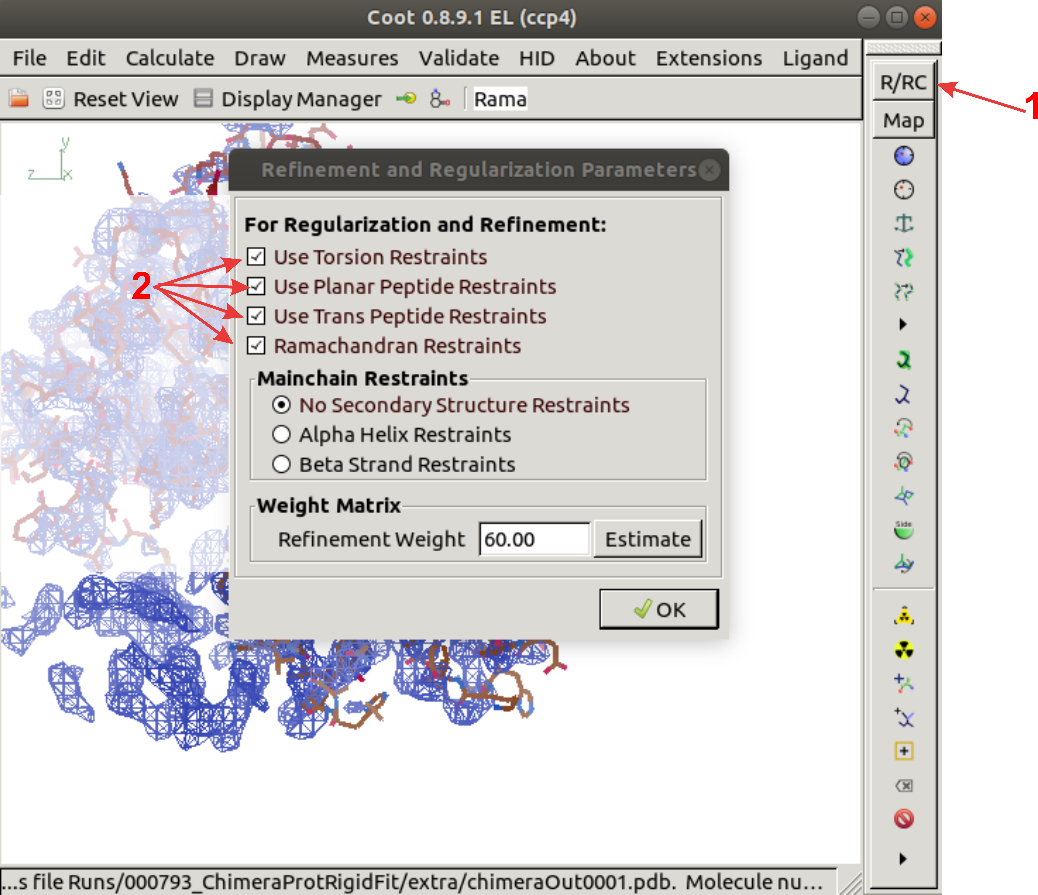
\includegraphics[width=0.80\textwidth]{Images_appendix/Fig121.pdf}
       \caption{Protocol \scommand{ccp4 - coot refinement}. \ttt{Refinement and regularization Parameters} window.}
       \label{fig:app_protocol_coot_3}
      \end{figure}
      
    \end{itemize} 
   
  Once those basic parameters are set, some steps to follow in refinement process are:
  \begin{itemize}
     \item Check validation parameter windows to have an idea of controversial areas and quality of the fitting:\\
     Go to \coot main menu \ttt{Validation -> Ramachandran Plot}, \ttt{Validation -> Density fit analysis} and \ttt{Validation -> Rotamer analysis}. Validation windows have to be checked throughout the refinement process.
     \item Refine the ends of each chain. Basic interactive refinement process requires several steps:
      \begin{itemize}
      \item First, go to an atom included in the area that is going to be refined:\\
      Go to \coot main menu \ttt{Draw -> Go To Atom...} and select chain and atom.
      \item Assess electron density in that area, and consider the possibility of processing part of the residues.
      \item Click the button \ttt{Real Space Refine Zone} (upper right side of \coot graphics window)  (\ffigure{fig:app_protocol_coot_4} (A) (1)) to put it active. Next, click two residues of the chain (2 and 3). A second flexible grey chain overlaps the starting chain. That grey chain can be moved in order to get a different conformation according to the density map (hidden in \ffigure{fig:app_protocol_coot_4} (A)). 
      \item If refinement parameters get acceptable values, press \ttt{Accept} in \ttt{Accept Refinement?} window (\ffigure{fig:app_protocol_coot_4} (B)).
     
      \begin{figure}[H]
       \centering 
       \captionsetup{width=.7\linewidth} 
       \includegraphics[width=0.80\textwidth]{Images_appendix/Fig122.pdf}
       \caption{Protocol \scommand{ccp4 - coot refinement}. (A) Interactive refinement of the chain fragment between residues 2 and 9. (B) Accepting refinement window.}
       \label{fig:app_protocol_coot_4}
      \end{figure}
     \end{itemize} 
     
    \item Refine each chain following instructions from Help section:
     \begin{itemize}
      \item Go to the residue \ttt{aaNumber} (\coot main menu \ttt{Draw -> Go To Atom...}).
      \item Initialize global variables.
      \item Repeat this loop until reaching the end of the chain:\\
      
        1.- Press \ttt{``z''} in the keyboard.\\
        2.- Inspect one by one, and fit to the volume density, every residue from the small auxiliary chain.\\
        3.- Accept the refinement.\\
       
      \item Check validation parameters to focus refinement in specific chain areas (\coot main menu \ttt{Validation ->  Density fit analysis}).
     \end{itemize} 
    \item After finishing refinement of every chain, save the structure (press \ttt{``e''} if \coot has to be definitively closed and not interactive anymore).
    \item Close \coot graphics window.
  \end{itemize}  

  
  \item Visualization of protocol results:
  
  After executing the protocol, press \ttt{Analyze Results} and \chimera graphics window will be opened by default. Atomic structures and volumes are referred to the origin of coordinates in \chimera. To show the relative position of atomic structures and electron density volumes, the three coordinate axes are represented; X axis (red), Y axis (yellow), and Z axis (blue) (\ffigure{fig:app_protocol_volume_3}). Coordinate axes, volume, and first atomic structure are model numbers \ttt{\#0}, \ttt{\#1}, \ttt{\#2}, respectively, in \chimera \ttt{Model Panel}. Every atomic structure saved during \coot refinement process will appear in \ttt{Model Panel} (\ffigure{fig:app_protocol_coot_5}). If you want to \underline{visualize results in \coot graphics window} you only have to open the protocol \underline{in the last point} that you let it before and \underline{set to \ttt{Continue}} the \ttt{Run mode}. Close the \coot protocol without saving anything in this case. 
  
  \begin{figure}[H]
    \centering 
    \captionsetup{width=.7\linewidth} 
    \includegraphics[width=0.80\textwidth]{Images_appendix/Fig123.pdf}
    \caption{Protocol \scommand{ccp4 - coot refinement}. \coot results visualized in \chimera.}
    \label{fig:app_protocol_coot_5}
   \end{figure}
   
  Since \scipion projects keep every intermediate atomic structure partially refined (\ffigure{fig:app_protocol_coot_6} (1, 3), users can include any of them in successive following modeling workflow steps performed in \scipion (\ffigure{fig:app_protocol_coot_7}).
  
  \begin{figure}[H]
    \centering 
    \captionsetup{width=.7\linewidth}  
    \includegraphics[width=0.80\textwidth]{Images_appendix/Fig124.pdf}
    \caption{Protocol \scommand{ccp4 - coot refinement}. Browse content after several runs of interactive \coot protocol.}
    \label{fig:app_protocol_coot_6}
   \end{figure}
   
   \begin{figure}[H]
    \centering 
    \captionsetup{width=.7\linewidth} 
    \includegraphics[width=0.50\textwidth]{Images_appendix/Fig125.pdf}
    \caption{Protocol \scommand{ccp4 - coot refinement}. \scipion window that allows to select any of \coot partially refined structures.}
    \label{fig:app_protocol_coot_7}
   \end{figure}
   
  \item Summary content:
  
   \begin{itemize}
     \item Protocol output (below \scipion framework) for each \coot intermediate atomic structure partially refined (\ttt{\#n}):\\ \ttt{ccp4 - coot refinement -> cootOut000\#n}; \ttt{PdbFile (pseudoatoms=False, volume=False)}.\\Pseudoatoms is set to \ttt{False} because the structure is made of atoms instead of pseudoatoms. Volume is set to \ttt{False} because no electron density map is associated to the atomic structure.
     \item \ttt{SUMMARY} box for each \coot intermediate atomic structure partially refined (\ttt{\#n}):\\\ttt{cootOut000\#n}:
    \end{itemize}
    
\end{itemize}


